\documentclass[conference]{IEEEtran}
%% SECON 2013 addition:
\makeatletter
\def\ps@headings{%
\def\@oddhead{\mbox{}\scriptsize\rightmark \hfil \thepage}%
\def\@evenhead{\scriptsize\thepage \hfil \leftmark\mbox{}}%
\def\@oddfoot{}%
\def\@evenfoot{}}
\makeatother
\pagestyle{headings} 

\ifCLASSINFOpdf
  % \usepackage[pdftex]{graphicx}
  % declare the path(s) where your graphic files are
  % \graphicspath{{../pdf/}{../jpeg/}}
  % and their extensions so you won't have to specify these with
  % every instance of \includegraphics
  % \DeclareGraphicsExtensions{.pdf,.jpeg,.png}
\else
  % or other class option (dvipsone, dvipdf, if not using dvips). graphicx
  % will default to the driver specified in the system graphics.cfg if no
  % driver is specified.
  % \usepackage[dvips]{graphicx}
  % declare the path(s) where your graphic files are
  % \graphicspath{{../eps/}}
  % and their extensions so you won't have to specify these with
  % every instance of \includegraphics
  % \DeclareGraphicsExtensions{.eps}
\fi
% *** MATH PACKAGES ***
%
\usepackage[cmex10]{amsmath}
\usepackage{amsfonts}
\usepackage{graphicx, epsfig}
\usepackage{color}
\usepackage{subfigure}
\usepackage{xspace}
\usepackage{algorithm}
\usepackage{algpseudocode}
\usepackage{breqn}
\usepackage{cite}
\usepackage{url}
\usepackage[export]{adjustbox}

\renewcommand{\thealgorithm}{}
\algnewcommand{\LineComment}[1]{\State \(\triangleright\) #1}
% A popular package from the American Mathematical Society that provides
% many useful and powerful commands for dealing with mathematics. If using
% it, be sure to load this package with the cmex10 option to ensure that
% only type 1 fonts will utilized at all point sizes. Without this option,
% it is possible that some math symbols, particularly those within
% footnotes, will be rendered in bitmap form which will result in a
% document that can not be IEEE Xplore compliant!
%
%\usepackage{array}
%\usepackage{mdwmath}
%\usepackage{mdwtab}
%\usepackage{eqparbox}
%\usepackage[tight,footnotesize]{subfigure}
%\usepackage[caption=false]{caption}
%\usepackage[font=footnotesize]{subfig}
%\usepackage[caption=false,font=footnotesize]{subfig}
%
%\usepackage{fixltx2e}

%\usepackage{stfloats}

%\usepackage{url}

% correct bad hyphenation here
\hyphenation{net-works}

\DeclareMathOperator*{\E}{\mathbb{E}}
\DeclareMathOperator*{\argmax}{arg\,max}

\begin{document}
%
% paper title
% can use linebreaks \\ within to get better formatting as desired
\title{Scalability, Delay Characterization, and Satisfiability of Quality-of-Information in Wireless Networks}

\IEEEoverridecommandlockouts

% author names and affiliations
% use a multiple column layout for up to three different
% affiliations

%\author{\IEEEauthorblockN{Scott Rager}
%\IEEEauthorblockA{Department of Computer Science and Engineering\\
%Pennsylvania State University\\
%University Park, PA 16802\\
%Email: rager@psu.edu}}

%\author{\IEEEauthorblockN{Scott Rager, Ertugrul Ciftcioglu, Thomas La Porta}
%\IEEEauthorblockA{Department of Computer Science\\
%and Engineering\\
%Pennsylvania State University\\
%University Park, PA 16802\\
%Email: rager@psu.edu, enc118@psu.edu, tlp@cse.psu.edu}
%\and
%\IEEEauthorblockN{Alice Leung, William Dron}
%\IEEEauthorblockA{Raytheon BBN Technologies\\
%Cambridge, MA 02138\\
%Email: aleung@bbn.com, wdron@bbn.com}
%\thanks{Research was sponsored by the U.S. Army Research Laboratory under the Network Science Collaborative Technology Alliance, Agreement Number W911NF-09-2-0053.} 
%}

%\author{
%  \IEEEauthorblockN{Scott T. Rager\IEEEauthorrefmark{1} \quad Ertugrul N. Ciftcioglu\IEEEauthorrefmark{2}  \quad Ram Ramanathan\IEEEauthorrefmark{3} \quad Thomas F. La Porta\IEEEauthorrefmark{1} \quad Ramesh Govindan\IEEEauthorrefmark{4} \\
%  }
%  \IEEEauthorblockA{
%  	\IEEEauthorrefmark{1}The Pennsylvania State University, University Park, PA 16802\\
%	\IEEEauthorrefmark{2}IBM Research, Yorktown Heights, NY 10598 \\
%  \IEEEauthorrefmark{3}Raytheon BBN Technologies, Cambridge, MA 02138 \\
%  \IEEEauthorrefmark{4}University of Southern California, Los Angeles, CA 90089
%  }
%
%  Email:  rager@psu.edu, enciftci@us.ibm.com , ramanath@bbn.com, tlp@cse.psu.edu, ramesh@usc.edu
%\thanks{Research was sponsored by the U.S. Army Research Laboratory under the Network Science Collaborative Technology Alliance, Agreement Number W911NF-09-2-0053.} 
%}


% for over three affiliations, or if they all won't fit within the width
% of the page, use this alternative format:
% 
%\author{\IEEEauthorblockN{Michael Shell\IEEEauthorrefmark{1},
%Homer Simpson\IEEEauthorrefmark{2},
%James Kirk\IEEEauthorrefmark{3}, 
%Montgomery Scott\IEEEauthorrefmark{3} and
%Eldon Tyrell\IEEEauthorrefmark{4}}
%\IEEEauthorblockA{\IEEEauthorrefmark{1}School of Electrical and Computer Engineering\\
%Georgia Institute of Technology,
%Atlanta, Georgia 30332--0250\\ Email: see http://www.michaelshell.org/contact.html}
%\IEEEauthorblockA{\IEEEauthorrefmark{2}Twentieth Century Fox, Springfield, USA\\
%Email: homer@thesimpsons.com}
%\IEEEauthorblockA{\IEEEauthorrefmark{3}Starfleet Academy, San Francisco, California 96678-2391\\
%Telephone: (800) 555--1212, Fax: (888) 555--1212}
%\IEEEauthorblockA{\IEEEauthorrefmark{4}Tyrell Inc., 123 Replicant Street, Los Angeles, California 90210--4321}}




% use for special paper notices
%\IEEEspecialpapernotice{(Invited Paper)}




% make the title area
\maketitle


\begin{abstract}
\boldmath
%area
%problem
Quality of Information (QoI) provides a context-dependent measure of the utility that a network delivers to its users by incorporating non-traditional information attributes.  
Quickly and easily predicting performance and limitations of a network using QoI metrics is a valuable tool for network design. Even more useful is an understanding of how network components like topology, bandwidth, protocols, etc. impact these limitations. 
%solution
In this paper, we develop a QoI-based framework that can provide this understanding of limitations and impact by modeling the various contributors to delay in the network, including channel rate and contention, competing traffic flows, and multi-hop propagation effects, and relating them to QoI requirements, especially completeness and timeliness.
%results
Analysis shows that large tradeoffs exist between network parameters, such as QoI requirements, topology, and network size.  Simulation results also provide evidence that the developed framework can estimate network limits with high accuracy.  Finally, this work also introduces  \emph{scalably feasible QoI regions}, which provide upper bounds on QoI requirements that can be supported for certain network applications.
%takeaway

\end{abstract}

% IEEEtran.cls defaults to using nonbold math in the Abstract.
% This preserves the distinction between vectors and scalars. However,
% if the conference you are submitting to favors bold math in the abstract,
% then you can use LaTeX's standard command \boldmath at the very start
% of the abstract to achieve this. Many IEEE journals/conferences frown on
% math in the abstract anyway.

% no keywords




% For peer review papers, you can put extra information on the cover
% page as needed:
% \ifCLASSOPTIONpeerreview
% \begin{center} \bfseries EDICS Category: 3-BBND \end{center}
% \fi
%
% For peerreview papers, this IEEEtran command inserts a page break and
% creates the second title. It will be ignored for other modes.
\IEEEpeerreviewmaketitle

\section{Finding Limits and Characterizing Delay}
\label{sec:delay_char}
As explained in Section \ref{sec:qoi_model}, delay of a flow can be expressed as
\begin{equation}
	D = \frac{ k_{req} \cdot I_S \cdot CF \cdot TF}{W} + \frac{P_S \cdot DF \cdot (PL-1)}{W}
\end{equation}
%We will make some substitutions to get the following version
%\begin{equation}
%	D = \frac{ P_S \cdot CF \cdot P_N \cdot TF}{W} + \frac{P_S \cdot DF \cdot (PL-1)}{W}
%\end{equation}
%
Let $PL()$ be a function that provides the path length between $i$ and $j$, and let $TF_{i}^{j}$ be a random variable of the Traffic Factor for the bottleneck node between $i$ and $j$, i.e. the node along the path from $i$ to $j$ with the highest $u_x$.  Finally, let $P_N$ be a random variable that describes the number of packets in a given request, capturing both the possible randomness of $k_{req}$ and $I_S$.  
Then, building on the equation for delay above and making some substitutions, we can get the following equation to describe the delay from a node $i$ given a destination of $j$:
\begin{equation}
	D_{i}^{j} = \frac{ P_S \cdot CF \cdot P_N \cdot TF_{i}^{j}}{W}  + \frac{P_S \cdot DF \cdot (PL(i,j)-1)}{W}
\end{equation}

%Also, recall that $TF$ is a random variable of the flows being forwarded at the bottleneck node along the path of the flow.  
Defining two constants to simplify the expression,
\begin{eqnarray*}
	C_1 = \frac{P_S \cdot CF}{W} \\
	C_2 = \frac{P_S \cdot DF}{W}
\end{eqnarray*}
we can express the delay as
\begin{equation}
	D_{i}^{j} = C_1 \cdot P_N \cdot TF_{i}^{j} + C_2 \cdot PL(i,j)
\end{equation}

We can develop an expression for a distribution of delay as follows.  First, we define the cumulative distribution of a source-destination pair $(i,j)$:
\begin{equation*}
	P( D_{i}^{j} \leq d ) = P( C_1 \cdot P_N \cdot TF_{i}^{j} + C_2 \cdot PL(i,j) \leq d )
\end{equation*}
\begin{equation*}
	= P( P_N \cdot TF_{i}^{j} \leq \frac{d - C_2 \cdot PL(i,j)}{C_1}  )
\end{equation*}
Next, conditioning over all possible values of $TF$, we get
\begin{equation*}
	P( D_{i}^{j} \leq d ) = \sum\limits_{\tau = 1}^{\tau_{max}} P( P_N \cdot TF \leq \frac{d - C_2 \cdot PL(i,j)}{C_1} | TF = \tau ) \cdot f_{TF_{i}^{j}}(\tau)
\end{equation*}
\begin{equation*}
	= \sum\limits_{\tau = 1}^{\tau_{max}} P( P_N \leq \frac{d - C_2 \cdot PL(i,j)}{C_1 \cdot \tau} ) \cdot f_{TF_{i}^{j}}(\tau)
\end{equation*}
Substituting the cumulative distribution representing the data load, $F_{P_{N}}$:
\begin{equation*}
	F_{D_{i}^{j}}(d) = \sum\limits_{\tau = 1}^{\tau_{max}} F_{P_N}( \frac{d - C_2 \cdot PL(i,j)}{C_1 \cdot \tau} ) \cdot f_{TF_{i}^{j}}(\tau)
\end{equation*}
Then, we can generalize the expression to give a distribution for a flow originating in node $i$ with an unknown destination by conditioning over all possible destinations, $j$.
\begin{equation}
\label{eq:delay_dist_pdf_i}
	F_{D_i} = \sum\limits_{j \neq i} [ \sum\limits_{\tau = 1}^{\tau_{max}} F_{P_N}( \frac{d - C_2 \cdot PL(i,j)}{C_1 \cdot \tau} ) \cdot f_{TF_{i}^{j}}(\tau) ] \cdot p(j)
\end{equation}
Finally, we can get an average distribution of all flows' delays by summing over all sources and dividing by the the number of sources.  This average delay distribution is in Equation (\ref{eq:full_delay_cdf}).

%\begin{figure*}[!t]
%\begin{equation}
%\label{eq:full_delay_cdf}
%	F_D(d) = \frac{1}{N} \cdot \sum\limits_{i = 1}^N \sum\limits_{j \neq i} \sum\limits_{tf=1}^{tf_{max}}  F_{P_N}( \frac{d - C_2 \cdot PL(i,j)}{C_1 \cdot p_N} ) \cdot f_{TF_{i | j}}( tf ) \cdot p(j)
%\end{equation}
%\end{figure*}

\begin{figure}[]
\centering
       \subfigure[Line Network, $N = 40$, $I_S = 36 KB$]{
%        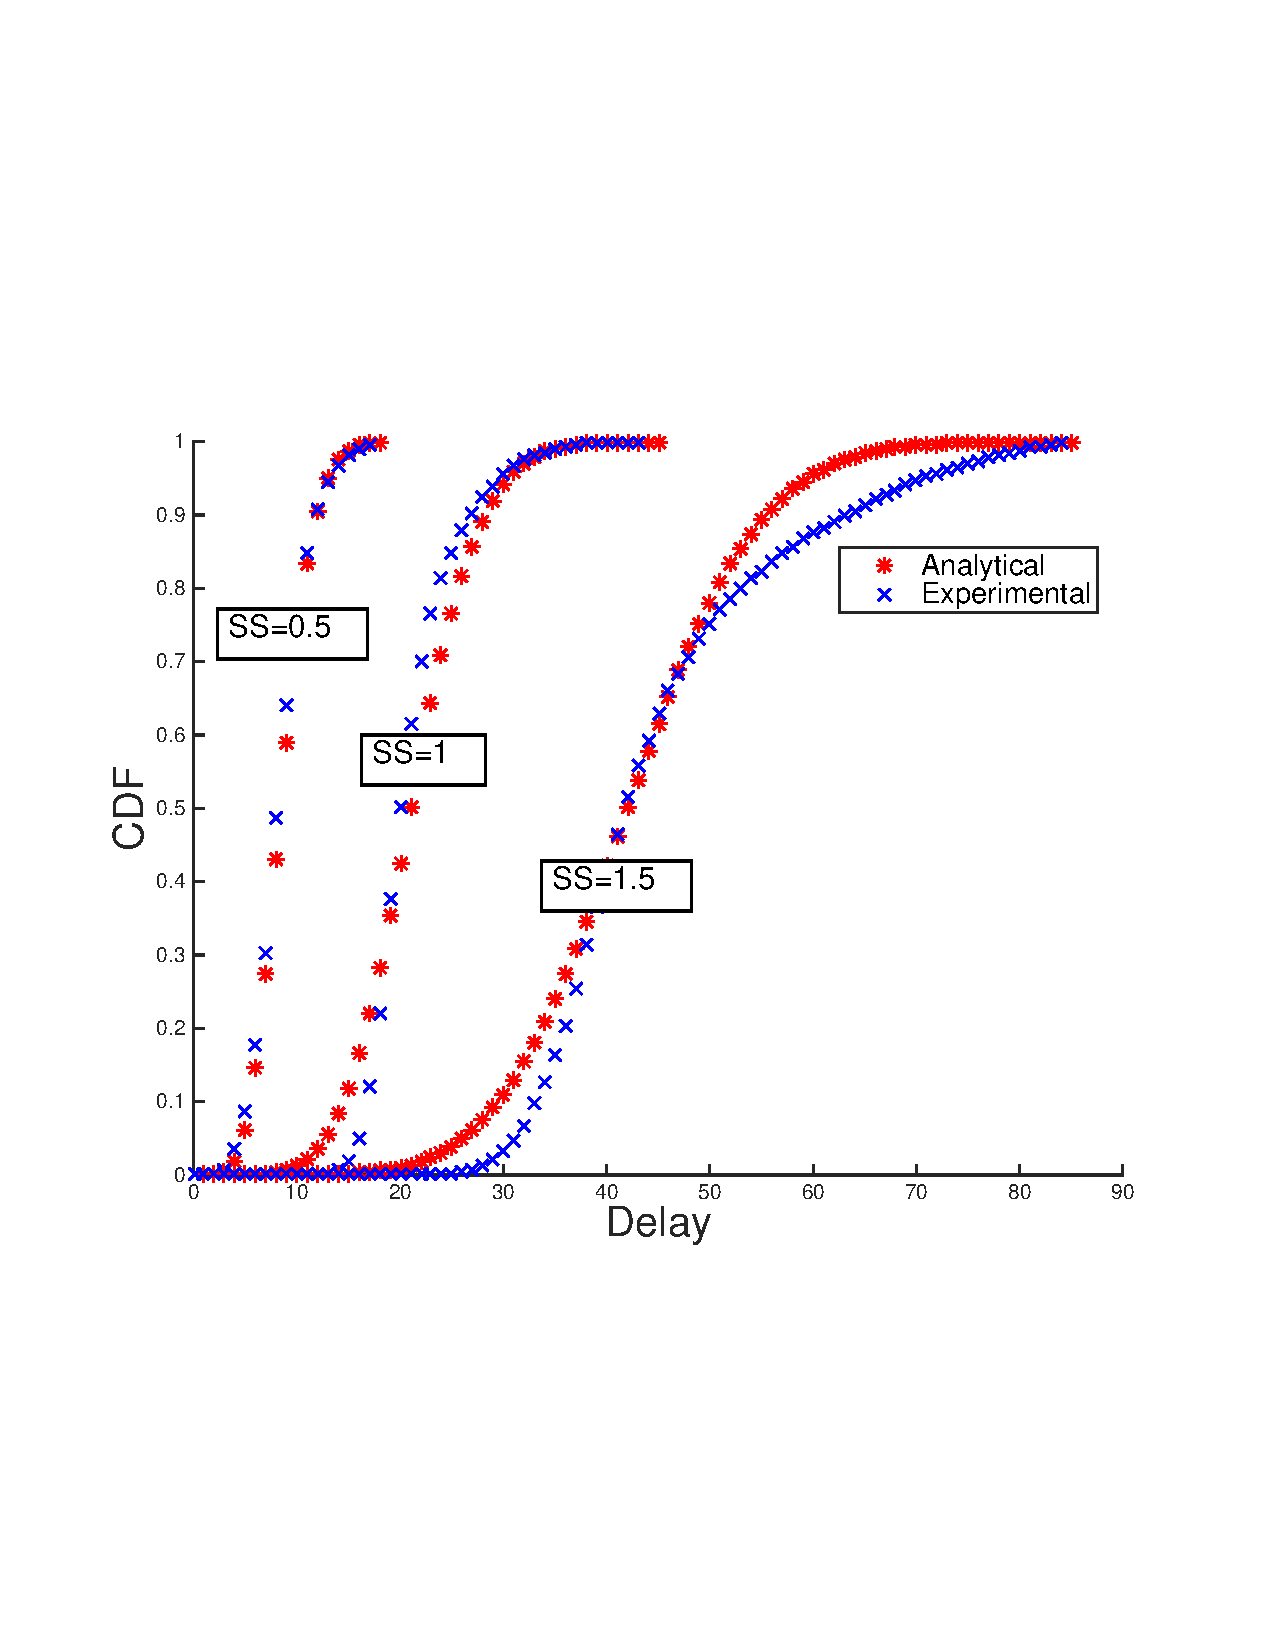
\includegraphics[scale=0.40, clip=true, trim=12mm 65mm 20mm 65mm]{figures/delay_cdfs/delay_cdf_line.pdf}
%        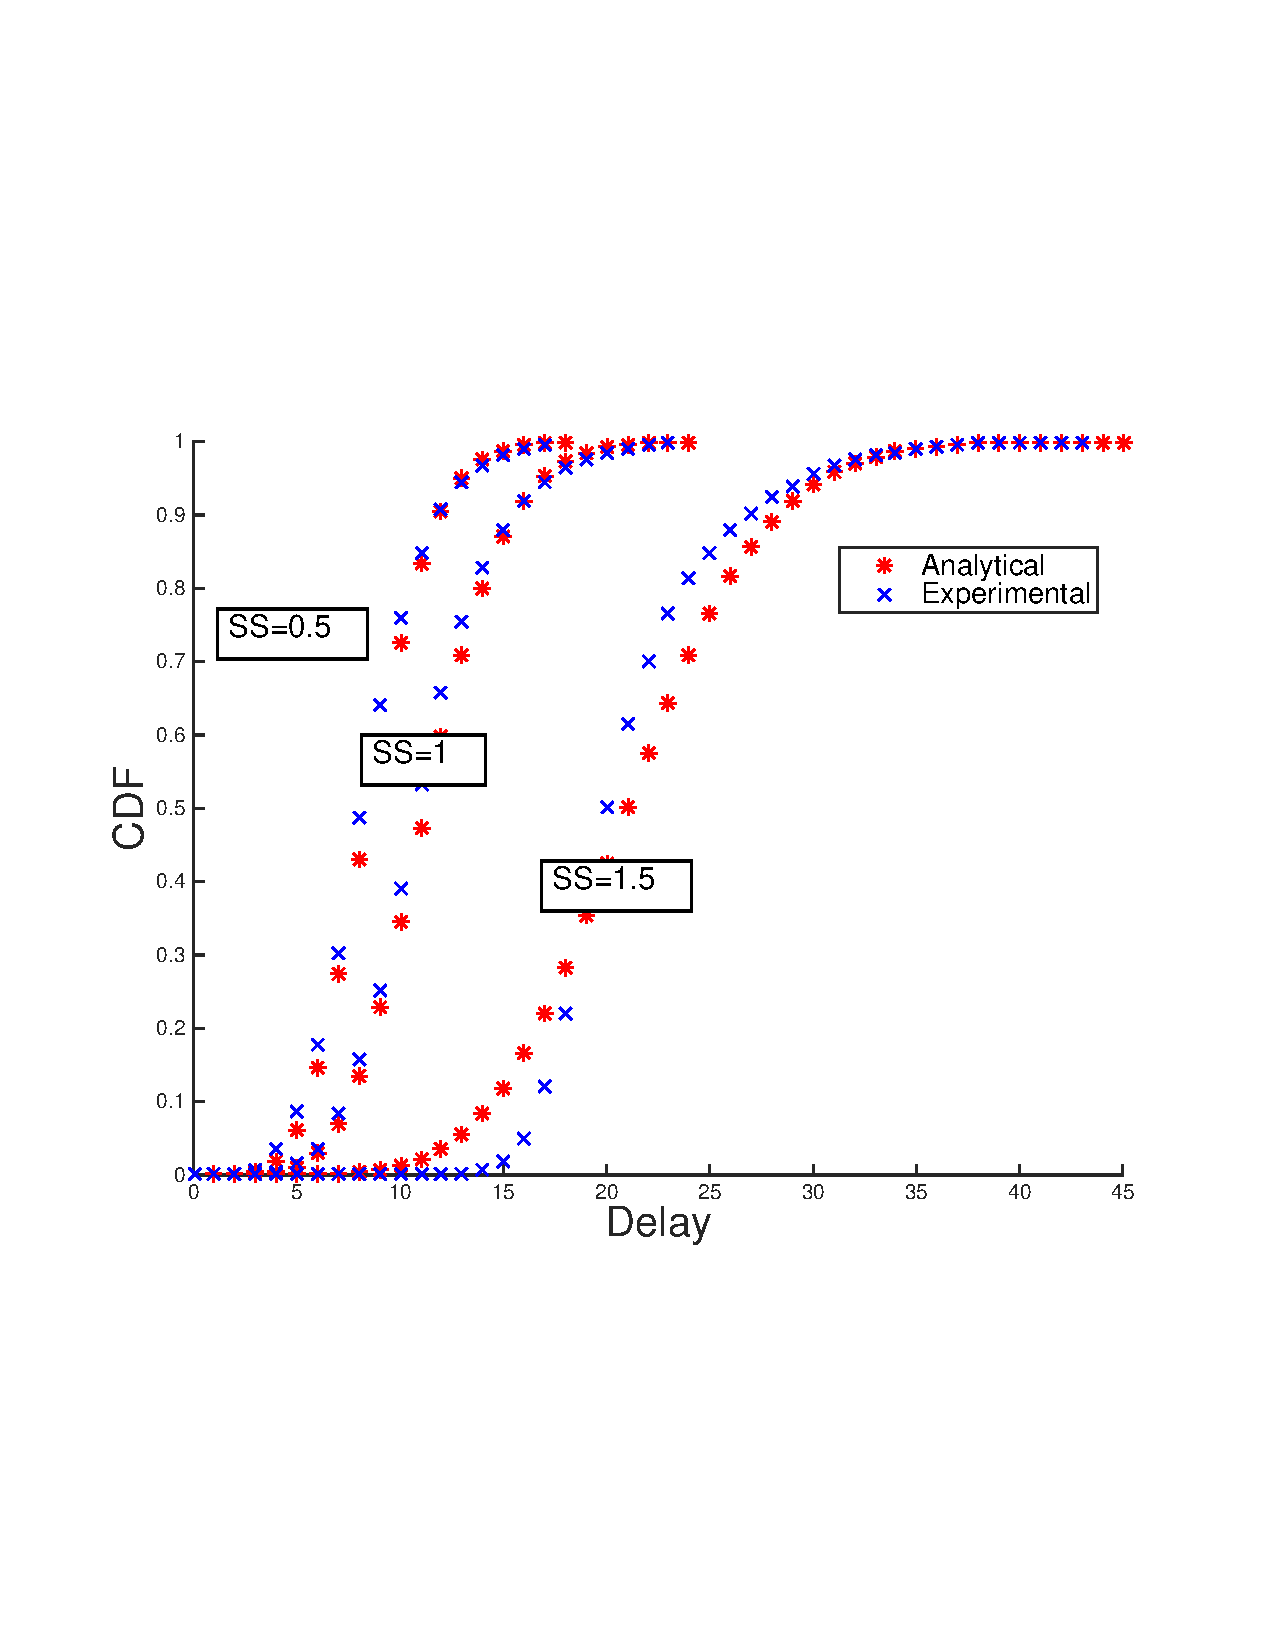
\includegraphics[scale=0.40, clip=true, trim=12mm 65mm 20mm 65mm]{figures/delay_cdfs/delay_cdf_line_full_2.pdf}
        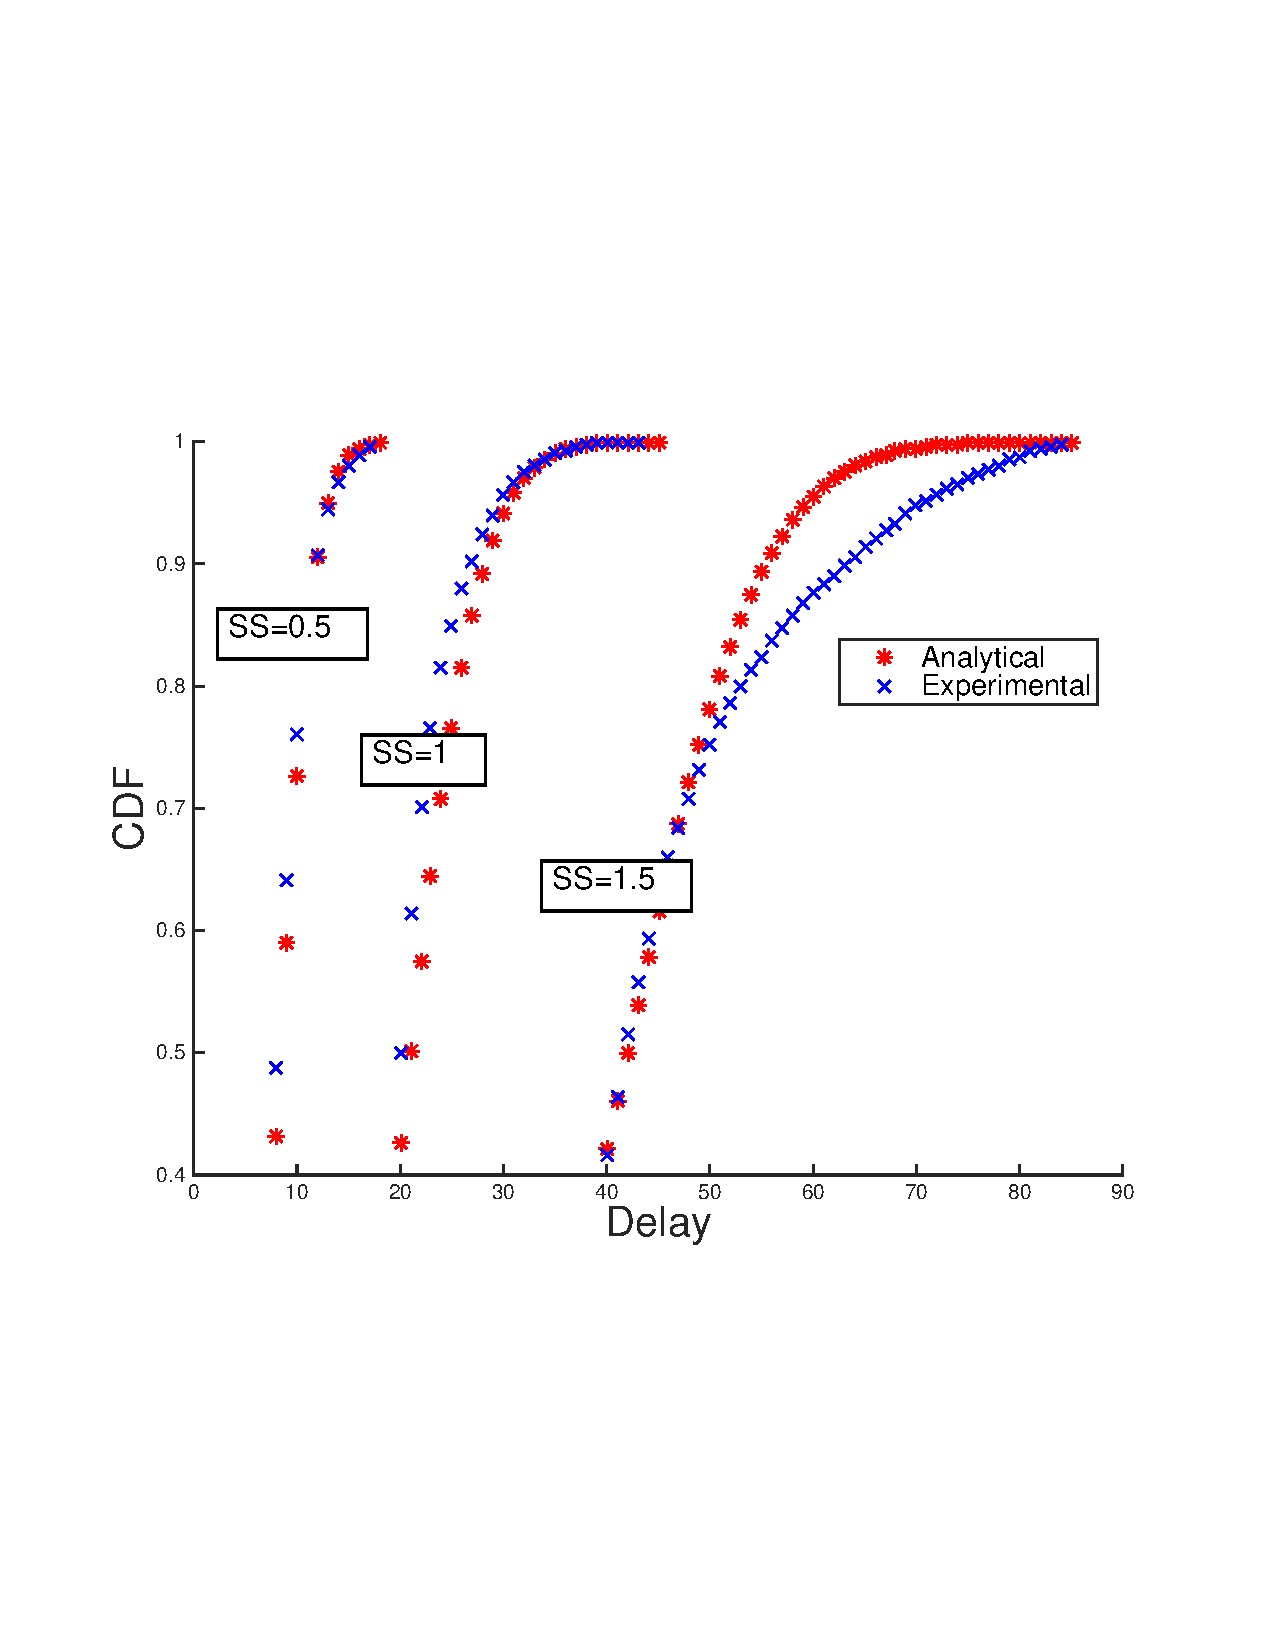
\includegraphics[scale=0.40, clip=true, trim=12mm 65mm 20mm 65mm]{figures/delay_cdfs/delay_cdf_line_half.pdf}
        \label{fig:scal_vs_qoi_line}
        }
    \subfigure[Grid Network, $N = 49$, $I_S = 72 KB$]{
%        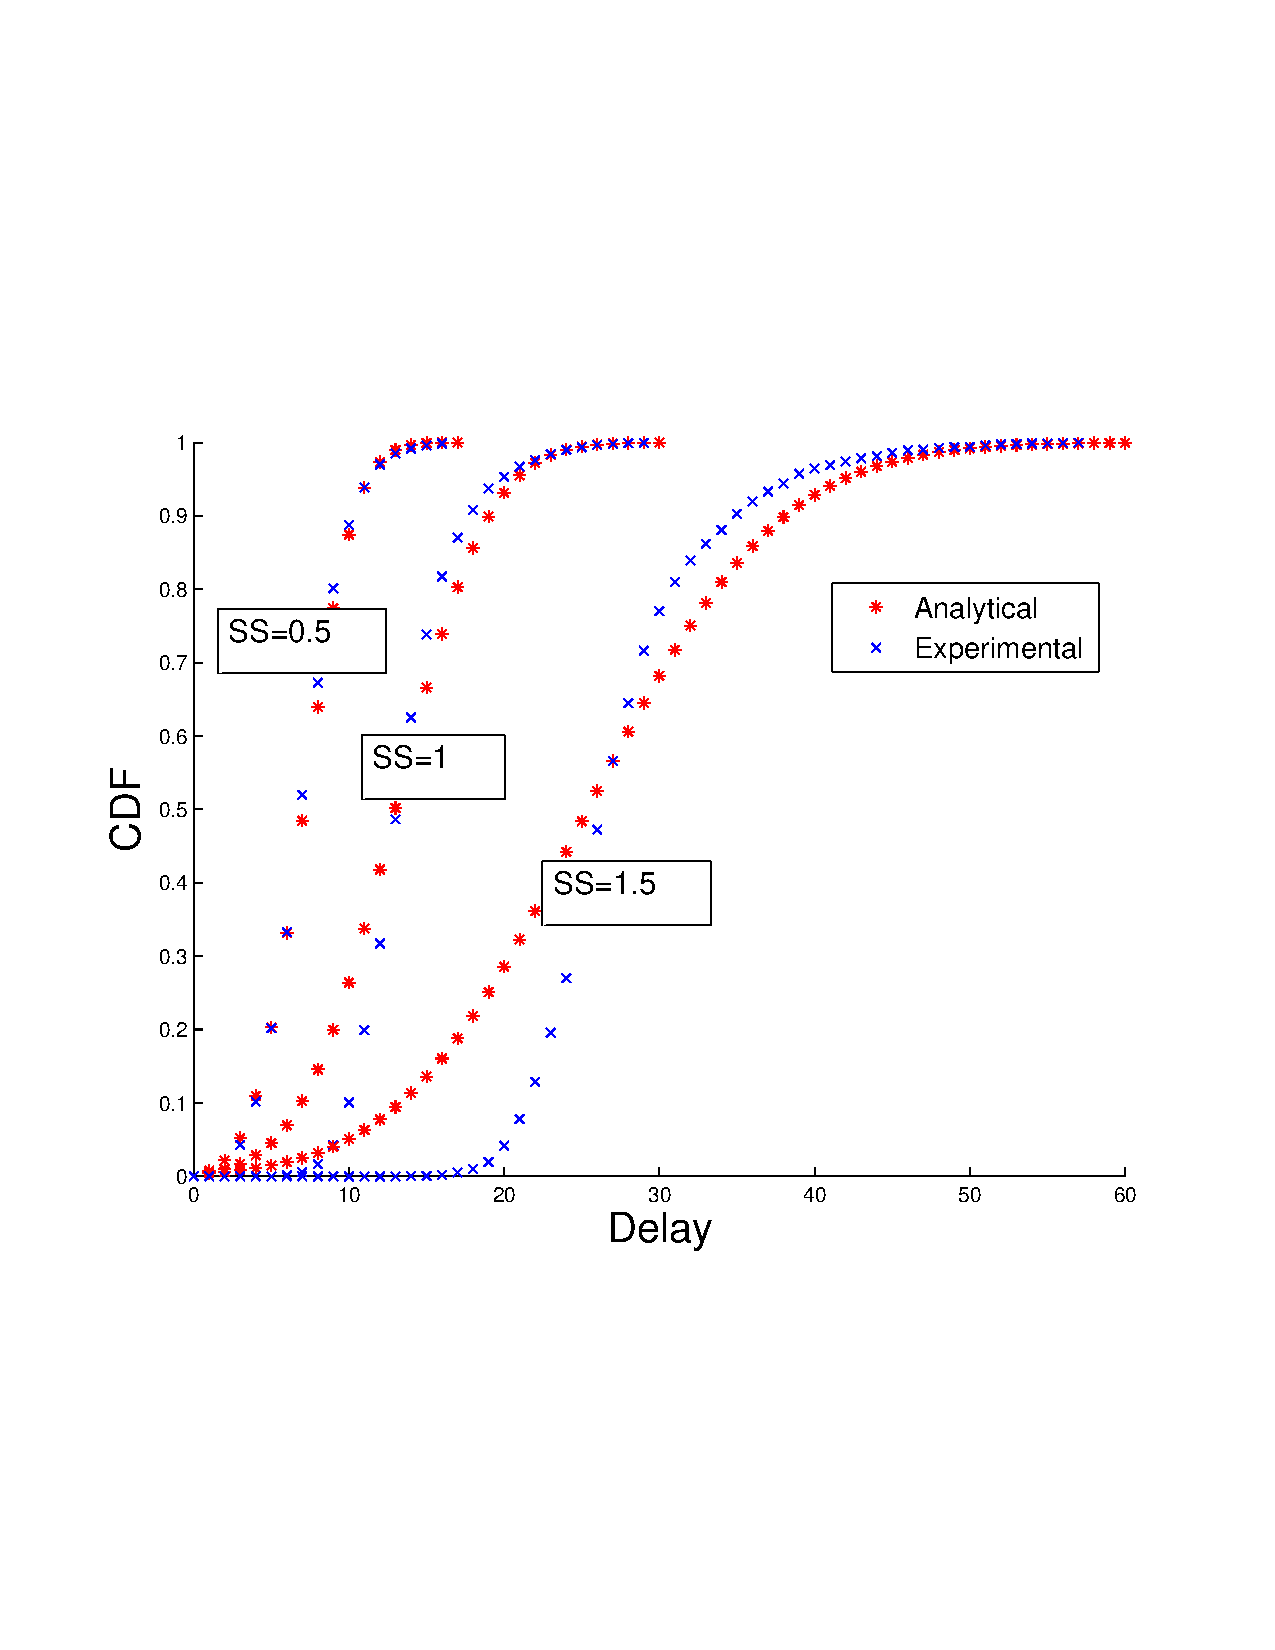
\includegraphics[scale=0.40, clip=true, trim=12mm 65mm 20mm 65mm]{figures/delay_cdfs/delay_cdf_grid.pdf}
        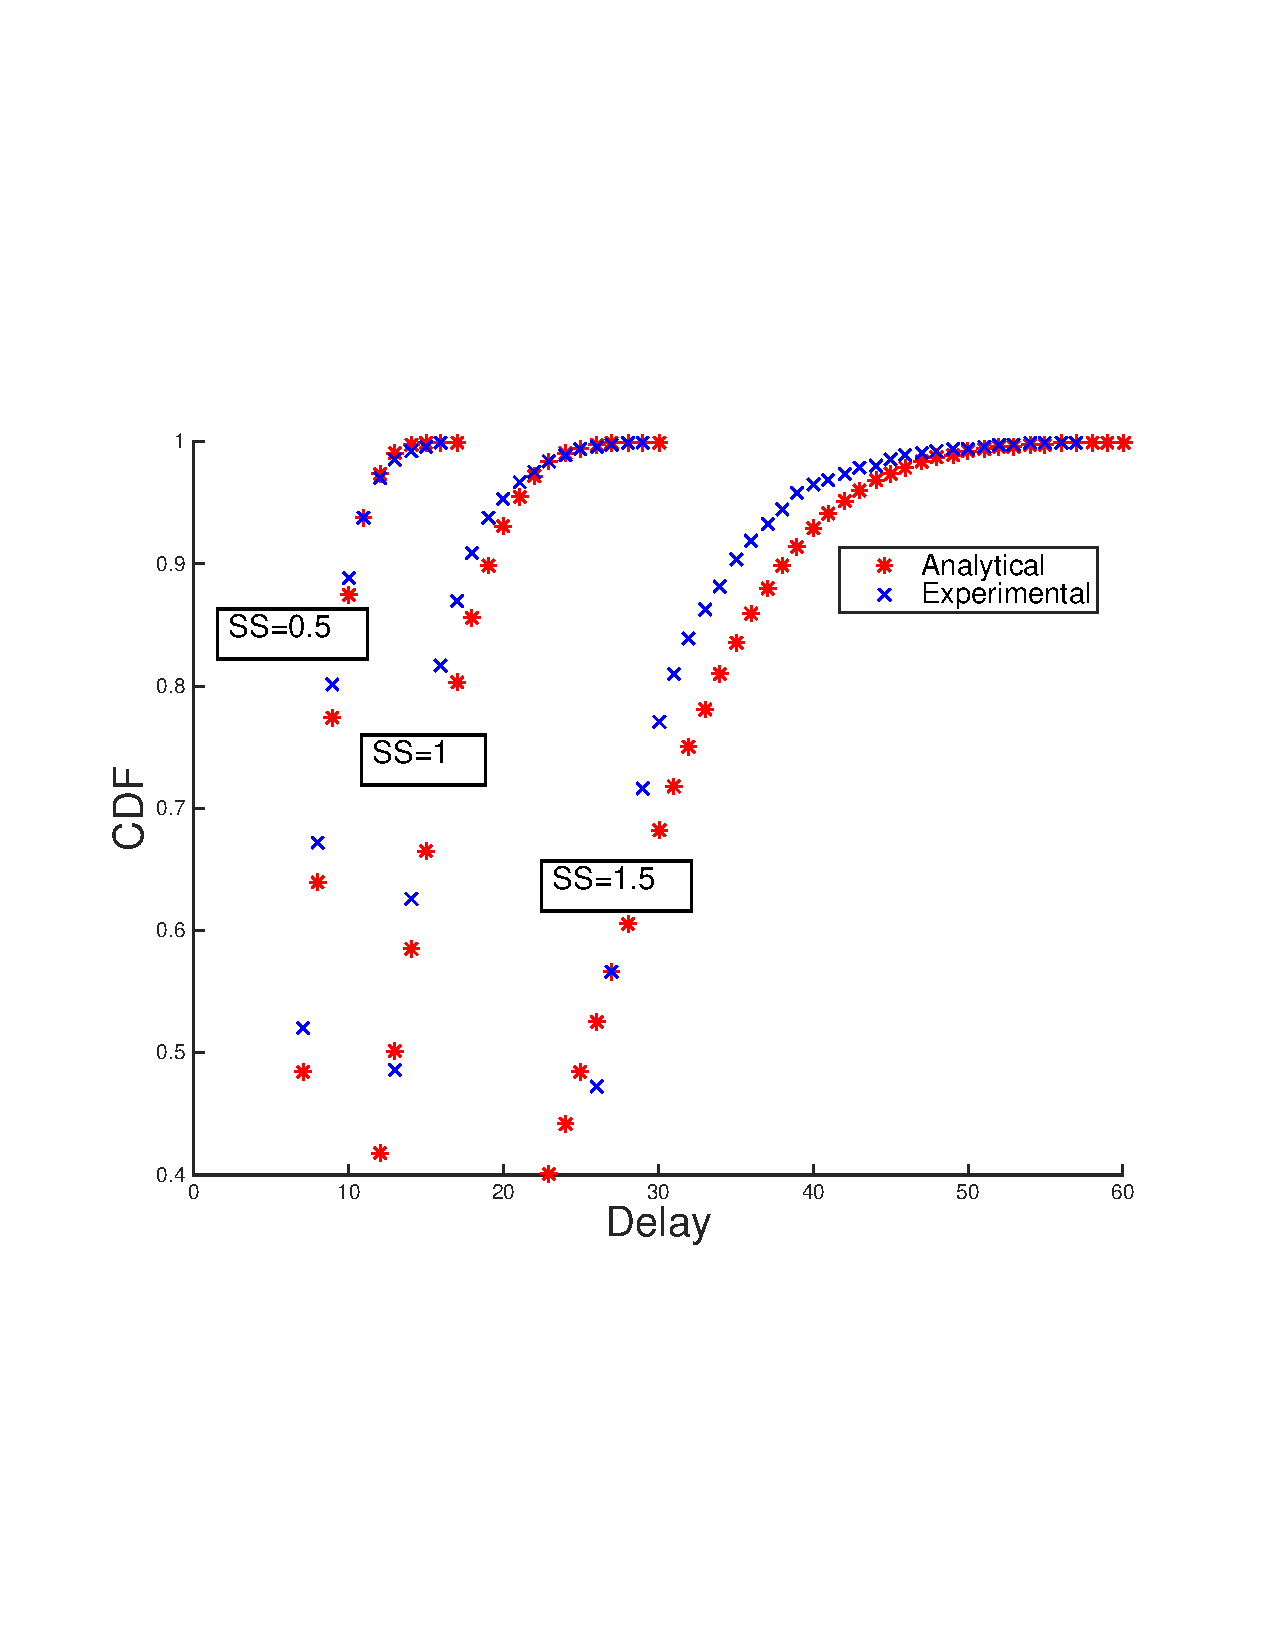
\includegraphics[scale=0.40, clip=true, trim=12mm 65mm 20mm 65mm]{figures/delay_cdfs/delay_cdf_grid_half.pdf}
        \label{fig:scal_vs_qoi_grid}
        }
   \caption{Characterization of delay using framework follows distribution of empirical results in most cases.}
   \label{fig:delay_cdf_anal_vs_sim}
\end{figure}

\subsection{Probability of Timeliness Satisfiability}

While the minimum timeliness at which all flows are expected to complete before their deadlines can be determined by the scalability equations in Section \ref{sec:example_applications}, some applications may benefit from an understanding of what the probability of completing within the timeliness constraints for those below the minimum fully satisfiable timeliness.  For example, if a mission issues a number of queries for information to support decision-making, receiving $80\%$ or $90\%$ of the responses may be sufficient for making the decision.  The question of importance, then, is "How far can we reduce the timeliness constraint and still expect to receive $x\%$ of the queries in time?"  Or, equivalently, we may pose the question, "When the network is operating at the edge of capacity, what is the expected delay for $x\%$ of queries to be completed?"  Since equation \ref{eq:full_delay_cdf} provides the distribution of delays, it provides quality estimates to answer these questions.  

\subsection{Validation of Delay Characterization}

Figure \ref{fig:delay_cdf_anal_vs_sim} shows expected delay distributions from \ref{eq:full_delay_cdf} alongside distributions of delays recorded in ns3 simulations of the same networks.  We argue that minimum QoI requirements for most applications tend to be over $50\%$, and therefore focus on the top half of the delay distribution.  In all cases here, analytical predictions of satisfying the timeliness requirement are within about $10\%$ of empirical results for probabilities above $0.5$.  

%Additionally, in smaller data load requirement cases, analytical predictions match simulation results quite closely along the entire distribution.

%\subsection{Scalability and Maximum QoI Equations}
%
%Once 

% from a different script:
%\subsubsection{Delay}
%
%The delay distribution for a flow beginning in source node $i$ is:
%
%\begin{equation}
%	f_{D_i} = \sum\limits_{j \neq i} [C_1 \cdot f_{TF_{i | j}}(tf) + C_2 \cdot PL(i,j)] \cdot p(j)
%\end{equation}
%which is equivalent to:
%\begin{equation}
%	P(D_i < d) = \sum\limits_{j \neq i} f_{TF_{i | j}}( \frac{d - C_2 \cdot PL(i,j)}{C_1} ) \cdot p(j)
%\end{equation}

%which can be expanded to:
%
%\begin{figure*}[t]
%\begin{eqnarray}
%\nonumber
%	f_{D_i} (d) = &&\frac{i}{N} \cdot \mathcal{N}( \frac{2(i-1)(N-i)}{(N-2)(N-1)} , \sqrt{\frac{2(i-1)(N-i)  (1-\frac{1}{N-1})}{(N-2)(N-1)}} )  \\ \nonumber
%			   &+& \sum\limits_{k=i}^{\frac{N}{2}-1} \cdot \frac{\frac{1}{2}-\frac{i}{N}}{\frac{N}{2} - i}\mathcal{N}( \frac{2(k-1)(N-k)}{(N-2)(N-1)}, \sqrt{\frac{2(k-1)(N-k)}{(N-2)(N-1)} (1-\frac{1}{N-1})} )  \\
%			   &+& \frac{1}{2} \cdot \mathcal{N} ( \frac{N(\frac{N}{2}-1)}{(N-2)(N-1)} , \sqrt{\frac{N(\frac{N}{2}-1)}{(N-2)(N-1)} (1-\frac{1}{N-1})} )
%\label{eq:full_PDF_TF_line_2}
%\end{eqnarray}
%\end{figure*}
% end from different script


%\appendix
%\input{sections/random_explanation}
% conference papers do not normally have an appendix


% use section* for acknowledgement
%\section*{Acknowledgment}


%The authors would like to thank...


% trigger a \newpage just before the given reference
% number - used to balance the columns on the last page
% adjust value as needed - may need to be readjusted if
% the document is modified later
%\IEEEtriggeratref{8}
% The "triggered" command can be changed if desired:
%\IEEEtriggercmd{\enlargethispage{-5in}}

% references section

% can use a bibliography generated by BibTeX as a .bbl file
% BibTeX documentation can be easily obtained at:
% http://www.ctan.org/tex-archive/biblio/bibtex/contrib/doc/
% The IEEEtran BibTeX style support page is at:
% http://www.michaelshell.org/tex/ieeetran/bibtex/
%\bibliographystyle{IEEEtran}
% argument is your BibTeX string definitions and bibliography database(s)
%\bibliography{IEEEabrv,../bib/paper}
%
% <OR> manually copy in the resultant .bbl file
% set second argument of \begin to the number of references
% (used to reserve space for the reference number labels box)
%\begin{thebibliography}{1}


\bibliographystyle{unsrt}

\bibliography{references}

%\bibitem{IEEEhowto:kopka}
%H.~Kopka and P.~W. Daly, \emph{A Guide to \LaTeX}, 3rd~ed.\hskip 1em plus
%  0.5em minus 0.4em\relax Harlow, England: Addison-Wesley, 1999.

%\end{thebibliography}




% that's all folks
\end{document}


